\documentclass{article}
\usepackage{cmap}
\usepackage[utf8]{inputenc}
\usepackage[english,ukrainian]{babel}
\usepackage{graphicx}
\usepackage{geometry}
\usepackage{listings}
\usepackage{float}
\geometry{
	a4paper,
	left=20mm,
	right=20mm,
	top=20mm,
	bottom=20mm
}
\lstset{
	language=c,
	tabsize=4,
	keepspaces,
	showstringspaces=false,
}
\graphicspath{ {./pictures} }
\setlength{\parindent}{4em}

\newcommand\subject{Алгоритми та структури даних}
\newcommand\lecturer{доцент кафедри ПЗ\\Коротєєва Т.О.}
\newcommand\teacher{асистент кафедри ПЗ\\Франко А.В.}
\newcommand\mygroup{ПЗ-22}
\newcommand\lab{3}
\newcommand\theme{Метод сортування Шелла}
\newcommand\purpose{Вивчити алгоритм сортування Шелла. Здійснити програмну реалізацію алгоритму сортування Шелла. Дослідити швидкодію алгоритму сортування Шелла}

\begin{document}
	\begin{normalsize}
		\begin{titlepage}
			\thispagestyle{empty}
			\begin{center}
				\textbf{МІНІСТЕРСТВО ОСВІТИ І НАУКИ УКРАЇНИ\\
					НАЦІОНАЛЬНИЙ УНІВЕРСИТЕТ "ЛЬВІВСЬКА ПОЛІТЕХНІКА"}
			\end{center}
			\begin{flushright}
				Інститут \textbf{КНІТ}\\
				Кафедра \textbf{ПЗ}
			\end{flushright}
			\vspace{200pt}
			\begin{center}
				\textbf{ЗВІТ}\\
				\vspace{10pt}
				До лабораторної роботи № \lab\\
				\textbf{На тему}: “\textit{\theme}”\\
				\textbf{З дисципліни}: “\subject”
			\end{center}
			\vspace{112pt}
			\begin{flushright}
				
				\textbf{Лектор}:\\
				\lecturer\\
				\vspace{28pt}
				\textbf{Виконав}:\\
				
				студент групи \mygroup\\
				Коваленко Д.М.\\
				\vspace{28pt}
				\textbf{Прийняв}:\\
				
				\teacher\\
				
				\vspace{28pt}
				«\rule{1cm}{0.15mm}» \rule{1.5cm}{0.15mm} 2022 р.\\
				$\sum$ = \rule{1cm}{0.15mm}……………\\
				
			\end{flushright}
			\vspace{\fill}
			\begin{center}
				\textbf{Львів — 2022}
			\end{center}
		\end{titlepage}
		
		\begin{description}
			\item[Тема.] \theme.
			\item[Мета.] \purpose.
		\end{description}
		
		\section*{Лабораторне завдання}
		Створити віконний проект та написати програму, яка реалізує алгоритм сортування Шелла.
		\begin{center}
			4. Задано матрицю дійсних чисел. Впорядкувати (переставити) її стовпці за зростанням значень їх перших елементів
		\end{center}
		
		\section*{Теоретичні відомості}
		Сортування Шелла (англійською «Shell Sort») — це алгоритм сортування, що є узагальненням сортування включенням.
		
		Алгоритм базується на двох тезах:
		
		Сортування включенням ефективне для майже впорядкованих масивів.
		Сортування включенням неефективне, тому що переміщує елемент тільки на одну позицію за раз.
		
		Тому сортування Шелла виконує декілька впорядкувань включенням, кожен раз порівнюючи і переставляючи елементи, що знаходяться на різній відстані один від одного. Сортування Шелла не є стабільним.
		
		Сортування Шелла названо начесть автора — Дональда Шелла, який опублікував цей алгоритм у 1959 році. 
		
		На початку обираються $m$ елементів: $d_1, d_2, …, d_m$, причому $d1 > d2 > … > d_m = 1$.
		
		Потім виконується m впорядкувань методом включення, спочатку для елементів, що стоять через $d_1$, потім для елементів через $d_2$ і так далі до $d_m = 1$.
		
		Значення   $d_1  = m/2$.
		
		Ефективність досягається тим, що кожне наступне впорядкування вимагає меншої кількості перестановок, оскільки деякі елементи вже стали на свої місця.
		
		Оскільки $d_m = 1$, то на останньому кроці виконується звичайне впорядкування включенням всього масиву, а отже кінцевий масив гарантовано буде впорядкованим. Час роботи залежить від вибору значень елементів масиву d. Існує декілька підходів вибору цих значень:
		
		Якщо $d$ — впорядкований за спаданням набір чисел виду $(2i  – 1) < n, j n$, то час роботи є $O(N1.5)$. Якщо $d$ — впорядкований за спаданням набір чисел виду $2i *3j < n/2, i, j n$, то час роботи є $O(Nlog2N)$.
		
		
		\subsection*{Покроковий опис роботи алгоритму сортування Шелла}
		\textbf{Алгоритм S - сортування Шелла}
		\begin{enumerate}
			\item [\textbf{S1}] Задаємо величину проміжку $= N/2$;
			\item [\textbf{S2}] Заходимо у внутрішній цикл, призначаємо $i = GAP$, поки $i < N$;
			\item [\textbf{S3}] Присвоюємо значення тимчасовій змінній $tmp=array[i]$;
			\item [\textbf{S4}] Заходиму у вкладений цикл, призначаємо $j=i+1$, поки $j<N$;
			\item [\textbf{S5}] Виконуємо порівняння поки $array[j-gap+1]>tmp$ інакше переставляємо елементи місцями $array[j]=array[j-gap+1]$, $j=j-GAP$;
			\item [\textbf{S6}] Повторити $S2$;
			\item [\textbf{S7}] Повторюємо зменшення проміжку $GAP=GAP/2$, поки $GAP > 0 $;
		\end{enumerate}
		
		\newpage
		
		\section*{Хід роботи}
		\subsection*{Файл sort.rs}
		\begin{lstlisting}
use crate::data::Data;

pub struct Sorted;

impl Sorted {
	pub fn sort(input: &mut Vec<Data>) -> Vec<Vec<Data>> {
		let len = input.len();
		let gaps = GapSequence::new(len);
		let mut res = vec![input.clone()];
		
		for gap in gaps {
			for i in gap..len {
				let mut j = i;
				
				while j >= gap && input[j - gap] > input[j] {
					input.swap(j - gap, j);
					res.push(input.clone());
					
					j -= gap;
				}
			}
		}
		res
	}
}

struct GapSequence {
	gap: usize,
}

impl GapSequence {
	fn new(n: usize) -> Self {
		Self { gap: n }
	}
}

impl Iterator for GapSequence {
	type Item = usize;
	
	fn next(&mut self) -> Option<usize> {
		self.gap /= 2;
		
		if self.gap > 0 {
			Some(self.gap)
		} else {
			None
		}
	}
}\end{lstlisting}
		
		\section*{Результат роботи}
		\begin{figure}[H]
			\centering
			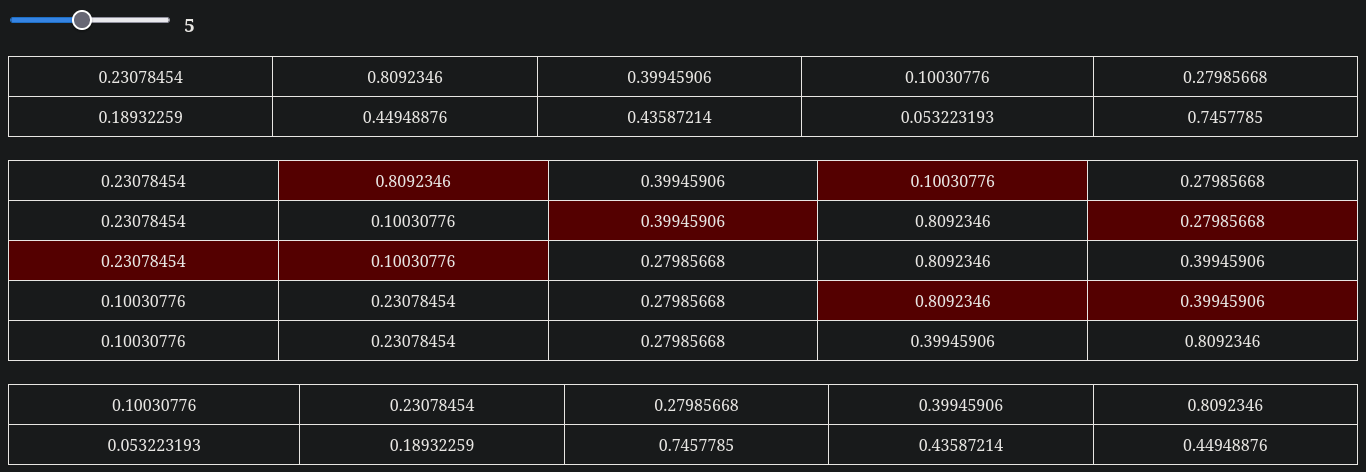
\includegraphics[scale=0.36]{1}
			\caption{Виконання програми}
		\end{figure}
		
		\section*{Висновок}
		Під час виконання лабораторної роботи я вивчив алгоритм сортування Шелла. Здійснив програмну реалізацію алгоритму сортування Шелла. Дослідив швидкодію алгоритму сортування Шелла.
		
	\end{normalsize}
\end{document}
